%!TEX root = ../main.tex
%%%%%%%%%%%%%%%%%%%%%%%%%%%%%%%%%%
% Links:
%
% Difficulty:
% Companies: 
%%%%%%%%%%%%%%%%%%%%%%%%%%%%%%%%%%


%\begin{figure}
%   \centering
%   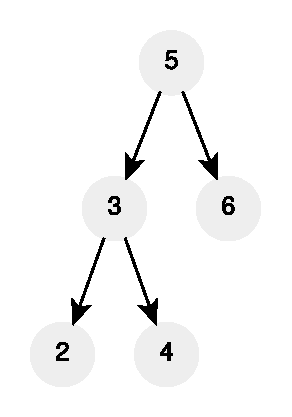
\includegraphics[width=\textwidth]{sources/count_numbers_conforming_bitmask/images/example1}
%   \caption[Sample short cpation]{Sample Caption}.
%   \label{fig:count_numbers_conforming_bitmask:example1}
%\end{figure}

\section{Count number integer conforming to any of the bitmasks}
\label{ch:count_numbers_conforming_bitmask}

\section{Problem statement}
\begin{exercise}
\label{example:count_numbers_conforming_bitmask:exercice1}
In this problem we consider unsigned 30-bit integers, i.e. all integers in the range $0,2^{30}$.
We say that integer $A$ conforms to integer $B$ if, in all positions where $B$ has bits set to $1$, $A$ has corresponding bits set to $1$.

For example $$00 0000 1111 0111 1101 1110 0000 1111 = 16244239$$ conforms to $$00 0000 1100 0110 1101 1110 0000 0001 = 13032961$$ while $$11 0000 1101 0111 0000 1010 0000 0101 = 819399173$$ does not conform to $$00 0000 1001 0110 0011 0011 0000 1111 =9843741$$

Write a function that given three 30-bit unsigned integers $A,B,C$ returns the number of unsigned 30-bit integers conforming to any among $A,B,C$.

    %example1
    \begin{example}
        \label{example:count_numbers_conforming_bitmask:example1}
        \hfill \\
        Given $$A = 11 1111 1111 1111 1111 1111 1001 1111 = 1073741727$$
        $$B = 11 1111 1111 1111 1111 1111 0011 1111 = 1073741631$$
        $$C = 11 1111 1111 1111 1111 1111 0110 1111 = 1073741679$$
        the function returns $8$. The following are the $8$ numbers comforming to $A$ or $B$ or $C$.
        \begin{itemize}
            \item  $11 1111 1111 1111 1111 1111 0011 1111 = 1073741631$
            \item  $11 1111 1111 1111 1111 1111 0110 1111 = 1073741679$
            \item  $11 1111 1111 1111 1111 1111 0111 1111 = 1073741695$
            \item  $11 1111 1111 1111 1111 1111 1001 1111 = 1073741727$
            \item  $11 1111 1111 1111 1111 1111 1011 1111 = 1073741759$
            \item  $11 1111 1111 1111 1111 1111 1101 1111 = 1073741791$
            \item  $11 1111 1111 1111 1111 1111 1110 1111 = 1073741807$
            \item  $11 1111 1111 1111 1111 1111 1111 1111 = 1073741823$
        \end{itemize}

    \end{example}

\end{exercise}


\section{Discussion}
\label{count_numbers_conforming_bitmask:sec:discussion}
Let's start by solving an easier version of this problem by trying to answer the following question: how many numbers are conformant to exactly a given unsigned $A$?
We know for sure that an integer $x$ must have its bit number $i$ set if $A$ bit number $i$ is set as well. However for every bit in $A$  that is \textbf{not} set we have a free choice between setting it or not. 
Because we have two choices for each of these positions, the total number of conformant numbers to $A$ is $2^{z}$ where $z$ is the number of bits not set in $A$.
For instance, there are exactly $4$ numbers that are conformant to $11 1111 1111 1111 1111 1111 0101 1111$ as we have two choices for the bit at index $5$ and two choices for the bit at index $7$.

What about the numbers that are simultaneously conformant to two numbers $A$ and $B$? In order for an unsigned to be conformant to both, it must be the case that $x$ has its bit at position $i$ set if either the bit at position $i$ in $A$ or $B$ is set (or in both).
If the bit at position $i$ is set in $A$ but not set in $B$, the bit at position $i$ in $x$ must still be set in order for it to be conformant to both $A$ and $B$, and we can see that the same is true if the bit at position $i$ is set in $B$ and not set in $A$ or when it is set in both $A$ and $B$. Regardless of the case, it must be set in $x$ if any between $A$ and $B$ has it set.
Now, we can extend this reasoning and say that a number $x$ is conformat to several numbers $A$,$B$,$C\ldots$ simultaneusly if $x$ is conformant to $A \: \vee \: B \: \vee C \:  \vee \: \ldots$ (where $\vee$ symbolizes the bitwise OR operation).

We can use this fact and build a solution around it if we realize that we can count all numbers that are conformant to $A$, $B$, and $C$ separately and add the results together as shown in Figure \ref{fig:count_numbers_conforming_bitmask:sets}. However by doing so we might count some numbers more than necessary and in particular, when adding together the number of numbers conformant to $A$ to the number of numbers conformant to $B$ we are counting the number of numbers conformant to $A$ \textbf{and} $B$ twice! The same reasoning applies for $A$ and $C$ and for $B$ and $C$ and for the number of numbers that are conformant to $A$, $B$ and $C$ simultaneously. These are counted three times.

From Figure \ref{fig:count_numbers_conforming_bitmask:sets} it is easy to visualize how many times each intersections of the sets $A,B$ and $C$ is counted and from there visualize that the final answer is:
$$ |A \cup B \cup C| = |A|+|B|+|C| - |A \cup B| - |A \cup C| - |B \cup C| + |A \cup B \cup C|$$. 
This is basically the inclusion-exclusion principle at work which generalizes the familiar method for counting the number of elements in the union of two finite sets.


An implementation of this idea is shown in Listing \ref{list:count_numbers_conforming_bitmask:incexl}.

\begin{figure}
    \centering
    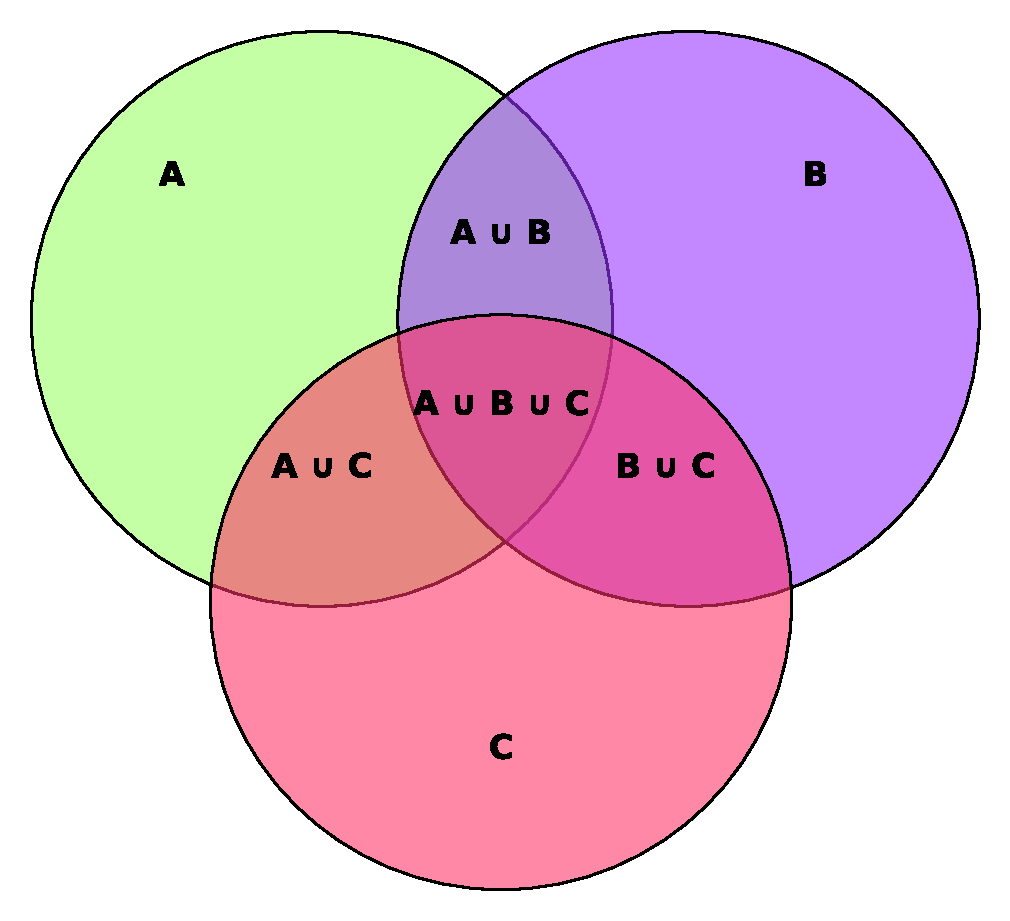
\includegraphics[width=\textwidth]{sources/count_numbers_conforming_bitmask/images/sets}
    \caption[]{Visualization of the inclusion-exclusion principle.}
    \label{fig:count_numbers_conforming_bitmask:sets}
\end{figure}

\subsection{Brute-force}
\label{count_numbers_conforming_bitmask:sec:bruteforce}

\lstinputlisting[language=c++, caption={Solution based on the inclusion-exclusion counting tecnique.},label=list:count_numbers_conforming_bitmask:incexl]{sources/count_numbers_conforming_bitmask/count_numbers_conforming_bitmask_solution1.cpp}

The function \inline{count_conforming} is responsible for counting the numbers conforming to just a single integer $N$ and it does so by counting the number of bits that are not set in $N$ which is equal to $30$ (the total number of bits in $N$) minus the number in $N$ that are set. To do so we use the function \inline{std::popcount} that is part of the \inline{<bit>} header is returns the number of $1$ bits in the argument (performs the same task as the GCC compiler intrinsic \inline{__builtin_popcount}).

